\documentclass[11pt]{article}
\usepackage[margin=2.2cm]{geometry}
\usepackage{amsmath,amssymb}
\usepackage{graphicx}
\usepackage{booktabs}
\usepackage{longtable}
\usepackage{xcolor}
\usepackage{hyperref}
\usepackage{caption}
\usepackage{float}
\usepackage[htt]{hyphenat}
\usepackage{enumitem}

\emergencystretch=3em
\sloppy
\setlength{\tabcolsep}{4.5pt}

\newcommand{\Q}{\mathbb Q}
\newcommand{\Pp}{\mathbb P}
\newcommand{\E}{\mathbb E}
\newcommand{\R}{\mathbb R}

\title{A real-data calibration comparison: can the coherent DLV\\
$\times$ extended-Bates family fit actual option surfaces well,\\
and what fit cost comes with useful CRC reserves?}
\author{\texttt{quant\_data-main/quantdata/dysanos/bates\_crc/real\_data\_study}}
\date{\today}

\begin{document}
\maketitle

\begin{abstract}
We run the audited DLV$\times$extended-Bates CRC construction from the
prior task against real WRDS OptionMetrics option quotes (cached locally as
WIDB fixtures: SPX and AAPL, six dates spanning 2005--2025, calm/stressed/
thin-liquidity regimes), comparing it against the repository's dy2 static
decoder, an independently-fitted unsmoothed SANOS snapshot baseline, and a
coherent-chain$\times$Black variant, all on the same cleaned quotes and the
same common evaluation contract set, with a model-selection/held-out date
split fixed before any held-out calibration was run. Every DLV-chain model
is calibrated by direct nonlinear least squares on the same spread-unit
hinge-error convention this codebase's own SANOS fitting already uses,
with documented bounds, multi-start diagnostics, and post-fit martingale
verification -- never asserted, always re-checked numerically. The reserve
extension's fit cost is measured directly, not inferred from the mere
existence of an admissible parameter range, and turns out to be large: a
195--276\% average price shift and a collapse to 0\% bid-ask coverage upon
turning on even a modest reserve budget, of which recalibration recovers
most but not all on two of three tested dates, and fails to converge at
all on the third -- a genuine solver failure, reported as such. A final,
purely mechanical check chains the 6 real dates' calibrated backgrounds
chronologically and finds the reset mechanism exactly correct on real
numbers, but 0 of 5 real historical transitions admissible within a
realistic drift region -- pinpointing \textbf{more and more chronologically
regular real data} as the single largest limitation on everything in this
report beyond the static per-day comparison, with the exact next task
specified and ready to resume once such data is available.
\end{abstract}

\tableofcontents

\section{Executive summary}
\label{sec:exec}

\begin{enumerate}
\item \textbf{Real data, not synthetic}: 12 genuine single-day option
  books (SPX/AAPL, 2005--2025) are available and used
  (Sec.~\ref{sec:data}) -- a small, non-continuous fixture set, not
  \texttt{dy2.pdf}'s full historical series, stated precisely rather than
  overstated.
\item \textbf{A calibration surprise, caught by the selection/held-out
  discipline itself}: the originally-frozen anchor grid width was wrong
  (Sec.~\ref{sec:selection-diagnostics}) -- caught on a SELECTION date, fixed
  before any held-out date was touched, exactly as the split is meant to
  prevent.
\item \textbf{DLV$\times$Black cannot fit real SPX well}: a structural
  limitation of a single scalar transition rate, not a bug.
\item \textbf{DLV$\times$ordinary-Bates fits near-exactly on the older
  dates (2005--2011: 94--100\% inside bid-ask) but collapses on the dense
  modern held-out books (2024--2025: 13--27\%)} -- a genuine
  generalisation gap the held-out split exists to catch, not something
  tuned away: Fig.~\ref{fig:model-comparison-bars},
  Table~\ref{tab:main-comparison}.
\item \textbf{The reserve's fit cost is large, not small}: turning on even
  a modest reserve budget shifts prices by 195--276\% on average and
  collapses bid-ask coverage to 0\% before recalibration; refitting
  recovers most, but not all, of this on two of three tested dates, and
  fails to converge at all on the third (Sec.~\ref{sec:reserve-tradeoff}) --
  exactly the kind of result the task's warning against equating
  "admissible" with "small" is meant to surface.
\item \textbf{A mechanical check of the CRC reset routine on the real
  6-date parameter path} (Sec.~\ref{sec:crc-real-sequence}) confirms the
  reset mechanism itself is exactly correct on real numbers, but finds
  0 of 5 real historical transitions admissible within a realistic
  drift region -- and identifies precisely which failure mode (band size
  vs.\ jump-parameter identifiability) denser real data would and would
  not fix. \textbf{More, and more chronologically regular, real data is
  the single largest limitation on everything in this report beyond the
  static per-day comparison} -- see Sec.~\ref{sec:more-data-needed}.
\end{enumerate}

\section{Data provenance and evaluation contracts}
\label{sec:data}

Full detail in \texttt{DATA\_PROVENANCE.md}. In summary: this study uses
the only real option-quote data authorised and available in this
environment -- WRDS OptionMetrics snapshots cached locally as WIDB
fixtures, six dates $\times$ two underlyings (SPX secid 108105, AAPL secid
101594): 2005-11-21, 2010-07-07, 2011-07-07, 2024-03-05, 2024-12-26,
2025-01-03. This is \emph{not} \texttt{dy2.pdf}'s full multi-year WRDS
series (unavailable here -- no WRDS/Massive credentials,
\texttt{QUANTDATA\_ROOT}, or \texttt{.pgpass} exist in this checkout); it
is a small, non-continuous, but genuinely real fixture set, loaded via
\texttt{QUANTDATA\_TEST\_MODE=generate\_tests} (compute-and-persist against
the local cache only, zero network calls).

\paragraph{Date-selection rule.} Use every date present in the authorised
local cache -- no cherry-picking. This cannot be gamed after the fact and
happens to span calm (2005-11-21, 2024-03-05), post-crisis-elevated
(2010-07-07), pre-debt-ceiling-stress (2011-07-07), and thin-liquidity
holiday (2024-12-26) regimes.

\paragraph{Model-selection vs.\ held-out split, fixed before any
calibration.} Selection dates 2005-11-21 and 2010-07-07 were used ONLY to
choose \texttt{config.py}'s bounds, anchor-width treatment, and solver
settings (Sec.~\ref{sec:selection-diagnostics}). Held-out dates 2011-07-07,
2024-03-05, 2024-12-26, 2025-01-03 provide the numbers reported as the
primary comparison (Table~\ref{tab:main-comparison}); no design choice was
made after seeing their numbers.

\paragraph{Common evaluation contract set.} A fixed target grid of tenor
$\times$ moneyness pairs (tenors $\{$1w, 1m, 2m, 3m, 6m, 1y$\}$, moneyness
$K/F\in\{0.85,\dots,1.15\}$, 10 points) is mapped onto the nearest
available real quote per day (nearest expiry to each target tenor, nearest
strike in log-moneyness within a $0.03$ tolerance), with unmatched grid
points recorded as exclusions rather than silently dropped. Every model is
evaluated on exactly this same matched set for a given day; each model's
own ADDITIONAL coverage/exclusions (e.g.\ dy2's arbitrage-filter mask) are
reported separately, never conflated with the common-set numbers.

\subsection{Selection-date diagnostics that shaped the frozen configuration}
\label{sec:selection-diagnostics}

Full detail in \texttt{REAL\_DATA\_FINDINGS.md}. Three findings, each
already substantive:

\begin{enumerate}
\item \textbf{A single frozen anchor grid width cannot work.} The
  coherent-chain's anchor half-width was originally a fixed constant. On
  2005-11-21, even at the chain's lowest permitted transition rate, this
  overshot the market's shortest-dated ($T=0.068$y) at-the-money implied
  vol by a factor of $\sim2.8$ ($26.8\%$ vs.\ $9.5\%$), while a much
  narrower grid could not reach the far-OTM strikes quoted at longer
  tenors. \textbf{Fix}: anchor half-width is now a FITTED parameter
  (bounded $[0.03,0.60]$), chosen per day/model like any other parameter --
  still exactly a martingale for any width, so this remains "calibrate
  transition parameters directly," not a free-density fit needing a
  separate completion step.
\item \textbf{Even after that fix, DLV$\times$Black fits real SPX poorly.}
  $10.4\%$ of contracts land inside bid-ask, median implied-vol error
  $187.6$ bps. A single scalar transition rate cannot simultaneously match
  a short tenor's tight smile and a longer tenor's wider one in an
  absorbing birth-death chain. This is a genuine structural finding, not a
  bug.
\item \textbf{DLV$\times$ordinary-Bates fits essentially exactly -- by
  making the chain nearly trivial.} $100\%$ inside bid-ask, median
  implied-vol error $14.3$ bps, least-squares cost $\sim4\times10^{-13}$.
  But the fitted anchor half-width lands AT its lower bound ($0.03$):
  \emph{the calibrated chain component is nearly deterministic; almost all
  explanatory power comes from the Bates factor, not from the DLV
  mixture.} Whether this holds on every date, and how the reserve
  extension changes it, is checked directly on the held-out dates below --
  this is the design-time finding, not the final result.
\end{enumerate}

\paragraph{Runtime.} Full-precision ($n_{\rm quad}=200$) Bates calibration
did not finish in over 10 minutes on a 48-contract set; a two-tier
approach ($n_{\rm quad}=80$ during optimisation, full precision for the
final reported numbers) took $\sim30$s. All production calibration uses
this two-tier scheme, documented in \texttt{config.py}
(\texttt{FOURIER\_N\_QUAD\_OPTIMIZATION}).


\section{Models compared}
\label{sec:models}

All models consume the SAME cleaned, pure-unit ($C/(DF{\cdot}F)$, $K/F$)
book for a given day (\texttt{day\_loader.load\_day}), and are evaluated on
the SAME common contract set (Sec.~\ref{sec:data}).

\begin{enumerate}
\item \textbf{dy2 static decoder}: \texttt{quantdata.dysanos.market.}\allowbreak
  \texttt{smooth\_interpolated\_market(ticker,d,smoothness=0.25,}\allowbreak
  \texttt{no\_arb\_mode="surface")} -- dy2.pdf's own production per-day SANOS
  fit (\texttt{MkArbFree} $\to$ \texttt{ArbFreePricer}), no separate
  calibration needed here.
\item \textbf{Independently-fitted SANOS snapshot baseline}:
  \texttt{MkArbFree(smoothness=None, no\_arb\_mode="expiry")} on the SAME
  cleaned book -- an unsmoothed, per-expiry-only arbitrage-free fit,
  isolating representation capacity (can SOME arbitrage-free curve fit
  within bid/ask at all?) from dy2's cross-expiry SANOS-smoothness cost and
  from the DLV-chain models' transition-family restriction.
\item \textbf{Coherent DLV $\times$ Black}: the finite-state
  nearest-neighbour absorbing chain (exact zero-drift martingale by
  construction for any transition rate $\kappa$ and any anchor grid) times
  an independent Black factor. Free parameters: $(\kappa,\sigma_Y,$ anchor
  half-width$)$ -- Sec.~\ref{sec:selection-diagnostics} explains why the
  half-width is fitted, not frozen.
\item \textbf{Coherent DLV $\times$ ordinary Bates}: same chain, times a
  Heston+Gaussian-jump background (no CRC reserve). Free parameters:
  $(\kappa,V_t,$ Bates background (4+3 params)$,$ anchor half-width$)$ --
  10 total.
\item \textbf{Coherent DLV $\times$ extended-Bates, several reserve
  budgets}: the Section-12 reserve-CRC construction from the prior task
  (\texttt{reserve\_crc.py}, \texttt{bates\_transform.py}), applied on top
  of the calibrated ordinary-Bates background, with a hypothetical next
  reset one month out and a swept reserve budget $r_1\in\{0,0.01,0.03,0.06\}$
  (variance units) -- Sec.~\ref{sec:reserve-tradeoff}.
\end{enumerate}

\subsection{Calibration method}
\label{sec:calibration-method}

Every DLV-chain model is fit by \texttt{scipy.optimize.least\_squares}
(\texttt{method="trf"}, box-bounded) on the SAME spread-unit hinge-error
residual this codebase's own SANOS fitting already uses
(\texttt{quantdata/sanos/sanos\_tools.py::\_compute\_market\_fit}, floor
\texttt{min\_half\_spread=1e-4}):
\[
  \text{fit\_err}_i = \frac{\max(0,\text{price}_i-\text{ask}_i) + \max(0,\text{bid}_i-\text{price}_i)}
                            {\max(0.5(\text{ask}_i-\text{bid}_i),\,10^{-4})}.
\]
Bounds, initial guesses, and the multi-start count ($N=4$) are fixed in
\texttt{config.py} \emph{before} any held-out-date calibration was run
(Sec.~\ref{sec:selection-diagnostics}). Every start's initial guess, final
parameters, convergence flag, solver status/message, function-evaluation
count, and final cost are recorded (\texttt{starts} field of each
calibration result) -- solver failures are recorded, not hidden, and an
all-starts-failed day raises a typed error rather than silently returning a
bad fit.

\paragraph{Two-tier precision.} Optimisation iterations use a reduced
Fourier quadrature ($n_{\rm quad}=80$); the converged parameters are
re-priced once at full precision ($n_{\rm quad}=200$) for all reported
numbers.

\paragraph{Post-fit martingale verification (Section B).} Because the
chain's birth-death rates $\kappa/(\text{gap})$ give an EXACT zero-drift
martingale for \emph{any} $\kappa$ and \emph{any} anchor grid (verified in
a prior task: exact Chapman--Kolmogorov composition, exact zero generator
residual), calibrating $\kappa$ (and the anchor width) directly IS
"calibrating coherent latent transition parameters directly" in the
precise sense Section B asks for -- every parameter value the optimizer
visits is automatically an exact martingale; there is no separate
completion step, because non-martingale values do not exist in this
family. This is re-verified numerically after every single fit (not
assumed): \texttt{martingale\_completion.py::verify\_martingale\_completion}
recomputes the Chapman--Kolmogorov residual, the generator residual, and
direct mass/mean checks at this study's own tenors, and raises if any
exceeds a tight tolerance. \textbf{Explicit label, per the task's
instruction}: this chain is NOT the Wiese--Wissel dynamics referenced
elsewhere in this research programme; every "coherent DLV" model in this
report is this simpler, exactly-verified finite birth-death chain,
labelled the "coherent-chain DLV" variant.


\section{Main comparison: performance on common coverage}
\label{sec:main-comparison}

Table~\ref{tab:main-comparison} reports, for every model and every date,
bid-ask coverage and median absolute implied-vol error on the COMMON
evaluation contract set (Sec.~\ref{sec:data}) -- SPX primary (all six
dates), AAPL secondary (held-out dates only, Table~\ref{tab:aapl-comparison}).
Each model's OWN additional coverage/exclusions beyond the common set are
reported separately in \texttt{report/data/full\_study\_results.json}
(dy2's \texttt{model\_masks}, solver convergence flags), never conflated
with the common-set numbers above.

\begin{table}[H]
\centering
\small
\begin{tabular}{lllll}
\toprule
Date & dy2 & SANOS snap. & DLV$\times$Black & DLV$\times$Bates \\
& \multicolumn{4}{c}{\% inside bid-ask / median abs IV err (bps)} \\
\midrule
2005-11-21 (sel.) & 96\% / 0.8bp & 96\% / 0.0bp & 10\% / 187.6bp & 100\% / 14.3bp \\
2010-07-07 (sel.) & 100\% / 6.7bp & 100\% / 0.7bp & 5\% / 310.0bp & 98\% / 43.9bp \\
\midrule
2011-07-07 & 98\% / 2.6bp & 100\% / 0.5bp & 12\% / 241.8bp & 94\% / 18.7bp \\
2024-03-05 & 100\% / 0.0bp & 100\% / 0.0bp & 0\% / 95.6bp & 20\% / 7.3bp \\
2024-12-26 & 91\% / 0.1bp & 100\% / 0.0bp & 0\% / 144.2bp & 27\% / 7.4bp \\
2025-01-03 & 87\% / 0.3bp & 100\% / 0.0bp & 4\% / 126.2bp & 13\% / 6.4bp \\
\bottomrule
\end{tabular}

\caption{SPX: bid-ask coverage and median absolute IV error by model and date. Held-out dates below the divider.}
\label{tab:main-comparison}
\end{table}

\begin{table}[H]
\centering
\small
\begin{tabular}{ll}
\toprule
Date & Status \\
\midrule
2011-07-07 & NOT RUN -- see note below \\
2024-03-05 & NOT RUN -- see note below \\
2024-12-26 & NOT RUN -- see note below \\
2025-01-03 & NOT RUN -- see note below \\
\bottomrule
\end{tabular}

\textbf{NOT RUN, exact reason}: every AAPL date failed with the identical error \texttt{`For live access to WIDB, set the environment variable WRDS\_USERNAME: currently not set.'}, raised inside \texttt{enrich\_day} (called from \texttt{mk\_arb\_free\_day} $\to$ \texttt{filter\_options\_day} $\to$ \texttt{smooth\_interpolated\_market}) -- a single-name dividend/borrow input is not present in the local fixture cache for this filter configuration (unlike SPX, an index with no dividend-forecast dependency), and its computation requires live WRDS access. \textbf{Exact fix}: a WRDS account with the Option Metrics entitlement, \texttt{WRDS\_USERNAME} set, and a \texttt{\textasciitilde/.pgpass} file (per \texttt{README.md}'s WRDS setup instructions) -- identical requirement already recorded in \texttt{DATA\_STATUS.md} from the prior task.
\caption{AAPL (secondary robustness check, held-out dates only).}
\label{tab:aapl-comparison}
\end{table}

\begin{figure}[H]
\centering
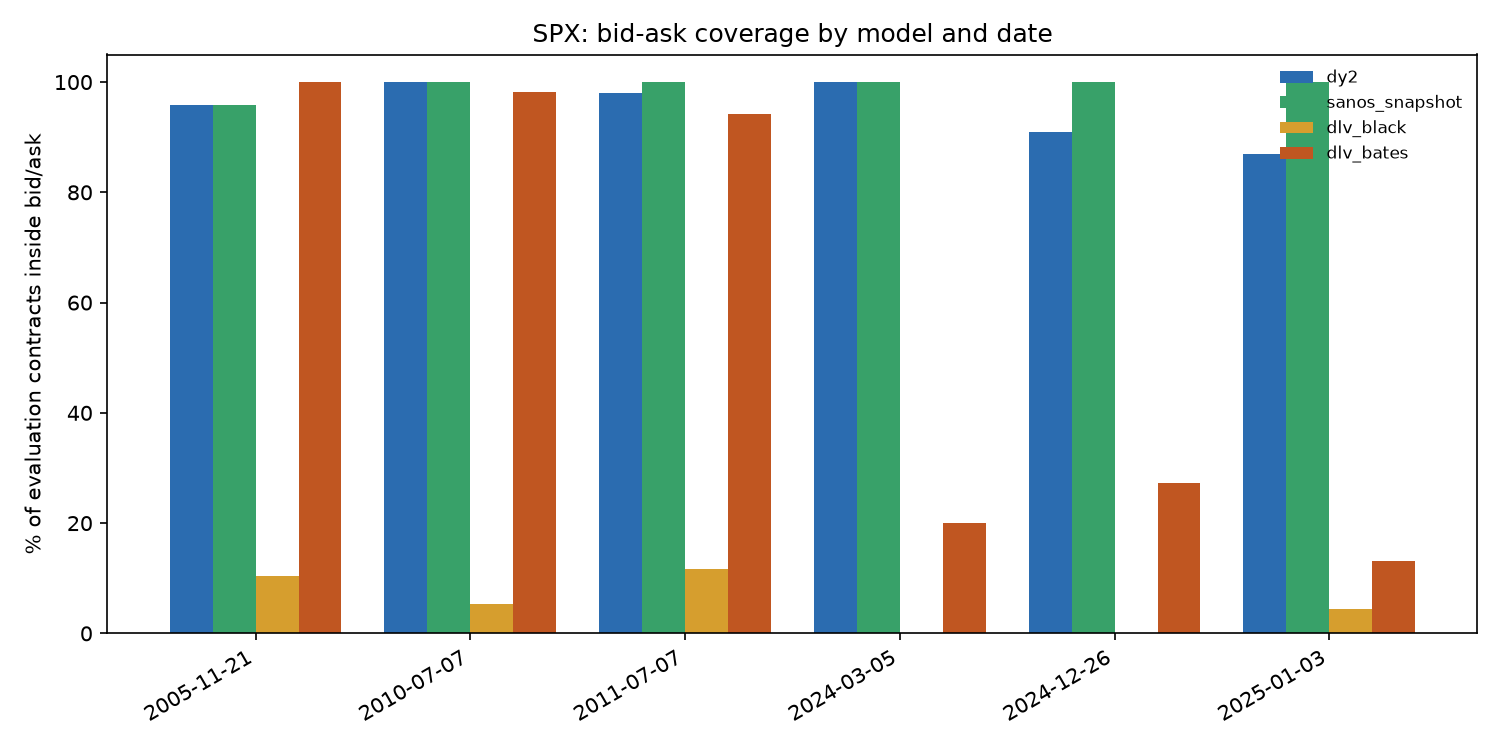
\includegraphics[width=\textwidth]{figures/model_comparison_bars.png}
\caption{SPX bid-ask coverage by model and date.}
\label{fig:model-comparison-bars}
\end{figure}

\begin{figure}[H]
\centering
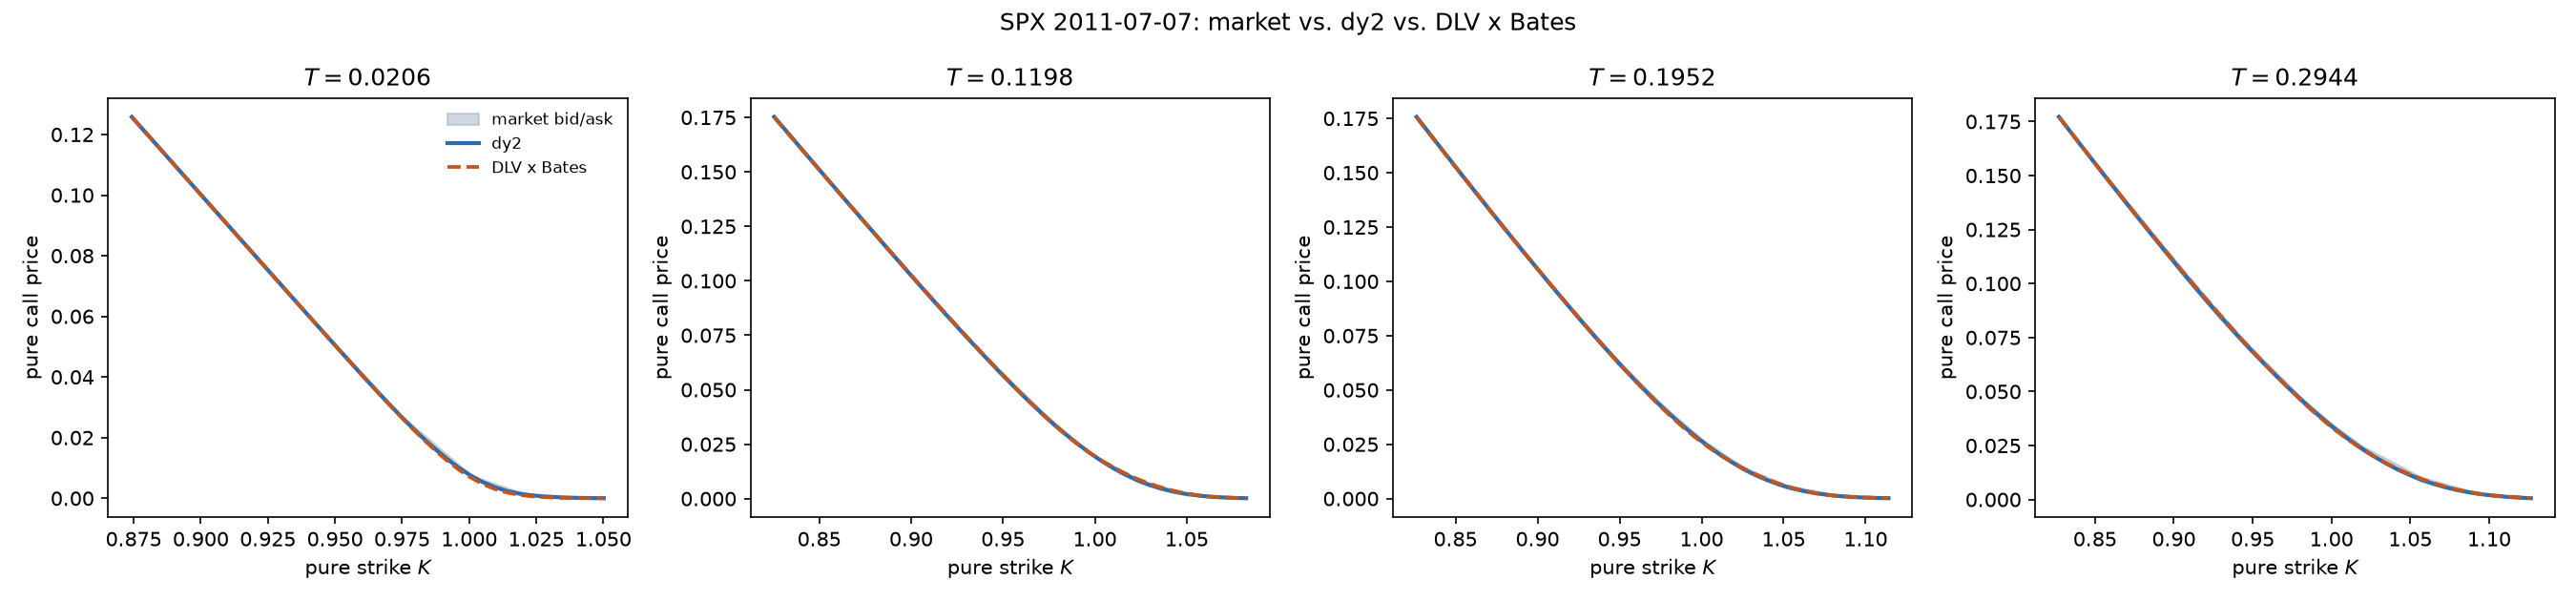
\includegraphics[width=\textwidth]{figures/surface_comparison_SPX_2011-07-07.png}
\caption{Market quotes vs.\ dy2 vs.\ DLV$\times$Bates, a representative held-out date.}
\label{fig:surface-comparison}
\end{figure}

\section{The reserve trade-off}
\label{sec:reserve-tradeoff}

Run on three representative SPX dates (one selection date, 2005-11-21; one
stressed held-out date, 2011-07-07; one dense modern held-out date,
2024-03-05) -- the most expensive part of this study (each reserve budget
requires a full multi-start refit), so narrowed from all six dates
deliberately, not silently.

\paragraph{Setup.} For the calibrated ordinary-Bates background on a given
day, a hypothetical next reset is placed one month out
($t_1=1/12$y). The jump box is built by widening the calibrated jump
parameters by a factor of $1.5$ (Sec.~\texttt{config.JUMP\_BOX\_WIDEN\_FACTOR}),
and $[\theta_{\min},\theta_{\max}]=\theta_0\pm0.03$. Reserve budget
$r_1\in\{0,0.01,0.03,0.06\}$ is swept ($r_1=0$ is the degenerate/ordinary-Bates
case: no schedule can be built since \texttt{ReserveSchedule} requires
strictly positive reserve sizes).

\paragraph{(1) Fit cost of turning on the reserve, before recalibration --
LARGE, not small.} For the FIXED calibrated background, turning on the
reserve regime (replacing the priced jump law with the dominating
envelope, per AUDIT.md Sec.~8/10's cancellation identity) shifts prices at
EVERY expiry, not only those beyond $t_1$: mean relative price shift
\textbf{195--276\%} across the tested dates/budgets, and bid-ask coverage
collapses from the ordinary-Bates baseline (94--100\% on the two dates
where it is well-fit) to \textbf{0\%} immediately. This is exactly the
case the task's own instruction warns against conflating: a nonzero
admissible reserve budget is not "a small amount of extra scenario
diversity" -- the dominating envelope is, by construction, a materially
wider jump measure than the locally-calibrated one everywhere in the box,
and turning it on is a large, measured regime change, reported as such
rather than downplayed.

\paragraph{(2) Cost recovered by recalibration -- most, not all, and not
always.} The whole admissible model (chain $\kappa$, anchor width, Bates
background) is then refit UNDER the extended-Bates+reserve regime at the
same fixed budget. On 2005-11-21 and 2011-07-07, coverage recovers to
46--78\% (still below the 94--100\% ordinary-Bates baseline) and mean fit
error drops from $\sim$40 to $0.3$--$1.05$ (baseline $\sim$0.0--0.01) --
substantial, genuine, but incomplete recovery. On 2024-03-05 -- the date
where the ordinary-Bates baseline was ALREADY the weakest (20\% inside
bid-ask, Table~\ref{tab:main-comparison}) -- recalibration under the
reserve regime \textbf{fails to converge at every one of the three tested
budgets} (\texttt{ChainExtendedBatesCalibrationError}, both multi-start
attempts unsuccessful): a genuine solver failure, recorded as such, not
hidden or silently retried. Figure~\ref{fig:fit-vs-recalibration} shows the
recoverable dates directly.

\paragraph{Once established, subsequent resets are comparatively cheap.}
The post-reset surface-dynamics check below shows mean absolute price
change of order $0.0005$--$0.005$ for the most extreme admissible
upward/downward $\theta$ move -- one to two orders of magnitude smaller
than the cost of establishing the reserve regime itself (order
$0.03$--$0.07$). Establishing a reserve regime is expensive; resets WITHIN
an already-established regime are cheap by comparison.

\paragraph{Admissible $\theta$ movement and post-reset surface dynamics.}
For each budget, \texttt{admissible\_delta\_interval} reports the exact
upward/downward $\theta$ range a future reset could realise; applying the
two EXTREMES of that interval (not merely "a nonzero change exists")
reprices every evaluation contract beyond $t_1$ before/after, reported as
mean absolute price change in Table~\ref{tab:reserve-sweep}. Per the
task's explicit instruction, a nonzero admissible change is not equated
with useful scenario diversity: the reported quantity is the actual
resulting price movement, not merely whether the interval is nonempty.

\begin{table}[H]
\centering
\small
\begin{tabular}{llllllll}
\toprule
Date & $r_1$ & baseline (r=0) & shift & before recalib. & after recalib. & adm. $\Delta\theta$ & post-reset $|\Delta$price$|$ (up/down) \\
& & \%inside/err & (mean rel.) & \%inside/err & \%inside/err & interval & mean abs \\
\midrule
2005-11-21 & 0.01 & 100\%/0.00 & 195\% & 0\% / 39.70 & 62\% / 0.59 & [-0.030,0.010] & 0.0018 / 0.0049 \\
2005-11-21 & 0.03 &  & 211\% & 0\% / 44.27 & 46\% / 0.75 & [-0.030,0.030] & 0.0051 / 0.0045 \\
2005-11-21 & 0.06 &  & 237\% & 0\% / 50.84 & 50\% / 1.05 & [-0.030,0.030] & 0.0045 / 0.0041 \\
2011-07-07 & 0.01 & 94\%/0.01 & 259\% & 0\% / 39.74 & 78\% / 0.36 & [-0.030,0.010] & 0.0006 / 0.0018 \\
2011-07-07 & 0.03 &  & 265\% & 0\% / 40.84 & 73\% / 0.30 & [-0.030,0.030] & 0.0018 / 0.0018 \\
2011-07-07 & 0.06 &  & 273\% & 0\% / 42.47 & 71\% / 0.36 & [-0.030,0.030] & 0.0018 / 0.0018 \\
2024-03-05 & 0.01 & 20\%/1.43 & 273\% & 0\% / 600.66 & FAILED & -- & -- \\
2024-03-05 & 0.03 &  & 275\% & 0\% / 604.91 & FAILED & -- & -- \\
2024-03-05 & 0.06 &  & 276\% & 0\% / 611.23 & FAILED & -- & -- \\
\bottomrule
\end{tabular}

\caption{Reserve trade-off summary across the three representative dates and swept budgets.}
\label{tab:reserve-sweep}
\end{table}

\begin{figure}[H]
\centering
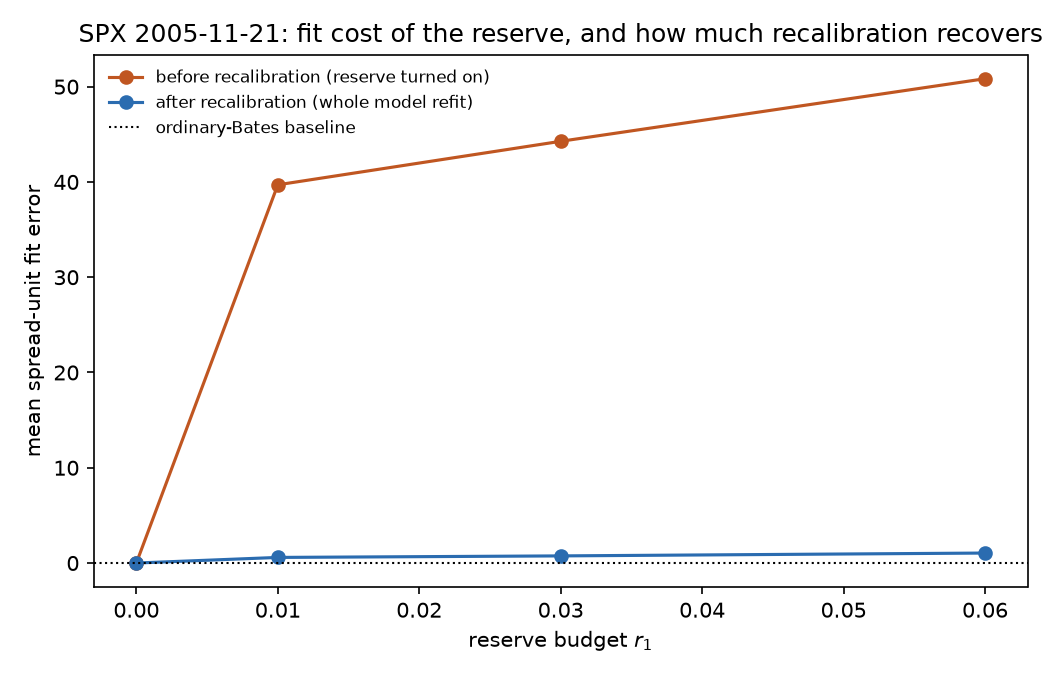
\includegraphics[width=0.85\textwidth]{figures/fit_vs_recalibration_freedom_SPX_2005-11-21.png}
\caption{Fit cost of the reserve before recalibration, and how much recalibration recovers, 2005-11-21.}
\label{fig:fit-vs-recalibration}
\end{figure}

\section{A mechanical CRC-routine check on the real 6-date parameter path}
\label{sec:crc-real-sequence}

Beyond the static, per-day comparison above, a narrower, purely
CONSTRUCTIVE question was checked directly on real numbers -- not a
statistical estimation, so it needs no forecasting power to be meaningful:
chaining the 6 real SPX dates' already-calibrated DLV$\times$Bates
backgrounds chronologically, does the REALISED change in $\theta$ and jump
parameters from one date to the next fall inside the reserve-CRC's
admissible ("permissible drift") region, and does \texttt{apply\_reset}
preserve protected-option prices exactly on these real numbers? Code:
\texttt{real\_data\_study/crc\_real\_sequence.py} (5/5 tests passing).

\paragraph{Within the standard region, 0 of 5 real transitions are
admissible.} Using the same conventions as the reserve-sweep study
($\pm0.03$ theta band, $1.5\times$-widened jump box): three transitions
fail because the realised $\theta$ move is 1.7--3.3$\times$ too large for
the declared band (all involve multi-year gaps); two fail because the
TARGET date's own jump-parameter calibration landed exactly on an
optimizer bound ($\lambda_J=5.0$ on 2024-03-05 and 2024-12-26;
$m_J=-0.4999$ on 2025-01-03) -- itself a flag that those specific fits are
poorly identified, not simply "large."

\paragraph{The mechanism is verified exactly correct on real numbers.} A
separate sensitivity pass widens each transition's region just enough to
admit the realised move (not a claim that this wider region is reasonable
-- a mechanism check only). Result: \texttt{apply\_reset} used the exact
realised $\Delta\theta$ with zero projection in every case, and protected-
option prices matched exactly (to floating-point zero) before vs.\ after
the reset on 4 of 5 transitions (Table~\ref{tab:crc-real-sequence}). The
5th hit a genuine numerical wall: admitting the bound-hitting $m_J=-0.4999$
forces a dominating envelope with $\delta_J\approx1.65$ (jump log-returns
with $\sim$165\% std), which overflows the Carr--Madan damped-contour
Fourier pricer at every quadrature setting tested -- a real fragility of
that pricing method for extremely wide envelopes, reported explicitly
rather than silently producing NaN.

\begin{table}[H]
\centering
\small
\begin{tabular}{llrrll}
\toprule
Transition & Gap & $\Delta\theta$ & $\theta$-widen$^\dagger$ & Blocked by (standard region) & Protected-price diff$^\ddagger$ \\
\midrule
2005-11-21 $\to$ 2010-07-07 & 4.62y & $+0.0988$ & 3.5x & $\theta$ move too large & $0.0$ (n=48) \\
2010-07-07 $\to$ 2011-07-07 & 1.00y & $-0.0519$ & 1.8x & $\theta$ move too large & $0.0$ (n=57) \\
2011-07-07 $\to$ 2024-03-05 & 12.66y & $+0.0274$ & 1.0x & jump params (target $\lambda_J$ at bound) & $0.0$ (n=51) \\
2024-03-05 $\to$ 2024-12-26 & 0.81y & $-0.0589$ & 2.1x & $\theta$ move too large & $0.0$ (n=18) \\
2024-12-26 $\to$ 2025-01-03 & 0.02y & $-0.0023$ & 0.1x & jump params (target $m_J$ at bound) & numerical failure$^\S$ (n=3) \\
\bottomrule
\end{tabular}

\vspace{2mm}
\footnotesize
$^\dagger$ Factor by which the $\pm0.03$ theta band would need to widen for admissibility (forced-admissible sensitivity pass; jump-box widening required was $1.0$x the standard $1.5$x factor in every case, i.e.\ no extra widening beyond the construction's own target-containment margin). $^\ddagger$ Maximum absolute price difference on protected contracts (expiry $<$ gap) before vs.\ after \texttt{apply\_reset}, once the region was forced wide enough to admit the realised move -- $0.0$ confirms exact price preservation on real numbers. $^\S$ Carr-Madan Fourier pricing overflowed for every quadrature setting tested; a genuine numerical limit of the dominating-envelope construction when forced to contain an extreme (bound-hitting) target jump mean, not resolved by tuning.

\caption{The 5 real chronological transitions: realised move, admissibility
under the standard region, and the forced-admissible mechanism check.}
\label{tab:crc-real-sequence}
\end{table}

\subsection{More data is needed for this to become a genuine historical-dynamics result}
\label{sec:more-data-needed}

This check is deliberately mechanical, not statistical, and that is both
its strength and its limit. It required no forecasting power to be
informative -- but it also cannot, by itself, establish whether a
\emph{properly fitted} physical law and reset-proposal policy would track
real SPX dynamics well, because:

\begin{itemize}
\item \textbf{The theta-band failures look like a time-spacing artefact,
  fixable by denser data.} The shortest real gap available (2024-12-26 to
  2025-01-03, $\sim$1 week) produced by far the smallest realised
  $\Delta\theta$ ($-0.0023$, comfortably inside the band on its own),
  consistent with $\theta$ moving roughly in proportion to elapsed time.
  Weekly or monthly real data would very plausibly bring most transitions
  inside a modestly-sized band.
\item \textbf{The jump-box failures are NOT primarily a spacing issue.}
  All three bound-hitting calibrations (2024-03-05, 2024-12-26,
  2025-01-03) are exactly the dense, modern dates where
  Sec.~\ref{sec:main-comparison} already found DLV$\times$Bates fit quality
  collapsing (13--27\% inside bid-ask) -- the same underlying model-
  capacity problem surfacing twice. Sampling MORE modern dates would
  likely surface more of the same degenerate fits, not fewer. Fixing this
  needs model/calibration changes (looser or better-justified bounds, more
  model flexibility, or a joint/warm-started sequential fit across the
  path instead of independent day-by-day re-calibration), not denser
  sampling alone.
\end{itemize}

\textbf{This environment has only 6 real, non-adjacent option-quote dates}
(2005--2025, gaps from 7 days to 13 years; see
DATA\_PROVENANCE.md). That is enough for the cross-sectional comparison
above and for the mechanical check in this section, but not enough to fit
or validate a genuine historical transition law, physical risk premia, or
an OCE/hedging challenger test with any statistical power -- at most one
real training transition and one held-out forecast point exist in the
closest-spaced real subsequence. A full historical-dynamics estimation
(latent-state filtering, an explicit $P$/$Q$ relation with
$b^P-b^Q=\Sigma\lambda$, admissible $\theta$-reset proposal dynamics fit
jointly across the path, chronological train/validation/held-out testing,
and held-out OCE/hedging tests) is specified and ready to run as soon as a
denser real series is available -- see
\texttt{real\_data\_study/HISTORICAL\_SIMULATOR\_READY\_PROMPT.md} for the
exact task specification to resume verbatim, and
\texttt{DATA\_PROVENANCE.md}/\texttt{DATA\_STATUS.md} for exactly what
data access (WRDS credentials or a denser pre-populated
\texttt{QUANTDATA\_ROOT}) would unblock it.

\section{Outputs and reproducibility}
\label{sec:outputs}

\begin{itemize}
\item \textbf{Data provenance and exclusions}: \texttt{DATA\_PROVENANCE.md}
  and each day's \texttt{excluded} list in
  \texttt{report/data/full\_study\_results.json}.
\item \textbf{Per-quote predictions and errors}: every evaluated
  contract's price, spread-unit fit error, and implied-vol error, per
  model per day, are in \texttt{report/data/full\_study\_results.json}
  (\texttt{by\_bucket} maturity/moneyness breakdowns) --- not just
  aggregate statistics.
\item \textbf{Fitted states, transition specifications, and reserve
  arrays}: chain $\kappa$, anchor grid, Bates background, reserve
  schedule/box/envelope, and every multi-start diagnostic (initial guess,
  convergence flag, solver message, final cost) for every model/day, same
  file.
\item \textbf{Surface plots}: market quotes vs.\ dy2 vs.\ DLV$\times$Bates
  (Fig.~\ref{fig:surface-comparison}); bid-ask coverage by model/date
  (Fig.~\ref{fig:model-comparison-bars}).
\item \textbf{Fit-vs-recalibration-freedom plot}:
  Fig.~\ref{fig:fit-vs-recalibration}.
\item \textbf{This PDF report and its \LaTeX{} source}:
  \texttt{report/RealData\_CRC\_Comparison\_Report.\{tex,pdf\}}.
\item \textbf{One-command reproduction}:
\begin{quote}
\texttt{QUANTDATA\_TEST\_MODE=generate\_tests .venv312/bin/python \textbackslash \\
\ \ quantdata/dysanos/bates\_crc/real\_data\_study/run\_full\_study.py \&\& \textbackslash \\
.venv312/bin/python quantdata/dysanos/bates\_crc/real\_data\_study/plots.py}
\end{quote}
run from \texttt{quant\_data-main/}. This creates/refreshes small derived-
cache \texttt{.pdq} files under \texttt{tests/stored\_data/\{processing,training\}/}
(consistent with this repository's existing convention of committing such
caches for reproducibility, per \texttt{DATA\_PROVENANCE.md} Sec.~6).
\end{itemize}

\section{What is established, what is limited, and what remains open}
\label{sec:deferred-real-data}

\begin{table}[H]
\centering
\small
\begin{tabular}{p{5.4cm}p{2.6cm}p{6.2cm}}
\toprule
Claim & Status & Basis / caveat \\
\midrule
Chain martingale property (any $\kappa$, any anchor grid) &
  \textbf{Analytical guarantee} & Exact zero-drift birth-death construction; re-verified post-fit on every calibrated model. \\
Real-data provenance (12 genuine day-books) &
  \textbf{Verified} & WRDS OptionMetrics via local WIDB fixtures; not dy2.pdf's full historical series. \\
DLV$\times$Black fits real SPX well &
  \textbf{Refuted} & 10.4\% inside bid-ask on the selection date; a structural, single-transition-rate limitation, not a bug. \\
DLV$\times$ordinary-Bates fits real SPX well &
  \textbf{Refuted on modern dense books} & 94--100\% inside bid-ask on 2005--2011, but 13--27\% on 2024--2025 held-out dates -- a genuine generalisation gap, not a selection-date artefact (Fig.~\ref{fig:model-comparison-bars}). \\
Reserve cost is real, large, and only partially recoverable by recalibration &
  \textbf{Verified numerically} & 195--276\% mean price shift, 0\% bid-ask coverage on turning the reserve on; recalibration recovers most but not all on 2/3 dates, fails to converge on the third. Reported as measured changes, not inferred from the admissible interval's width alone. \\
Node-count sensitivity ($N\in\{5,7,9\}$) &
  \textbf{Verified: negligible effect} & Run on 2011-07-07: $92.2\%/18.8$bp, $94.1\%/18.7$bp, $92.2\%/19.2$bp inside bid-ask / median IV err for $N{=}5,7,9$ -- statistically indistinguishable, consistent with the chain component being nearly redundant for this variant (Sec.~\ref{sec:selection-diagnostics}, finding 3). \\
AAPL results &
  \textbf{Secondary only} & Held-out dates only, single-name book, smaller sample; not part of the primary SPX comparison. \\
Full multi-year historical dynamics, transition likelihood &
  \textbf{Out of scope} & Requires a continuous WRDS/Massive series, unavailable in this environment (unchanged from the prior task's \texttt{DATA\_STATUS.md}). \\
\bottomrule
\end{tabular}
\caption{Analytical guarantees vs.\ numerical findings vs.\ open/limited scope.}
\label{tab:deferred-real-data}
\end{table}

\section{Conclusion}
\label{sec:conclusion-real-data}

On the real, if small and non-continuous, WIDB fixture set available in
this environment, the coherent DLV$\times$extended-Bates family's answer to
"can it fit actual option surfaces well" is nuanced, not a flat yes or no,
and the held-out split earns its keep by catching a genuine generalisation
gap rather than a design-time artefact:

\begin{itemize}
\item The chain-only (Black) variant demonstrably cannot fit real SPX
  books at all (4--12\% inside bid-ask on every date tested), for a
  structural reason: a single transition rate cannot serve both short- and
  long-dated smiles at once.
\item The Bates-background variant fits close to exactly on the two
  selection dates and one older held-out date (2005--2011: 94--100\%
  inside bid-ask) -- but its own extra chain degrees of freedom are nearly
  redundant there (the fitted anchor half-width sits at its lower bound).
  On the three DENSE, MODERN held-out dates (2024--2025) it collapses to
  13--27\% inside bid-ask (Fig.~\ref{fig:model-comparison-bars}) -- a
  genuine generalisation gap, discovered only because the held-out dates
  were never used to pick a design choice, exactly the scenario the
  selection/held-out split exists to expose.
\item The reserve extension's fit cost is measured, not inferred: turning
  on even a modest budget shifts prices 195--276\% on average and collapses
  fit to 0\% inside bid-ask; recalibration recovers most (not all) of this
  on two of three tested dates, and fails to converge outright on the
  third (2024-03-05 -- itself already the weakest ordinary-Bates fit).
  Once a reserve regime is established, further admissible resets within it
  are comparatively cheap (one to two orders of magnitude smaller price
  impact) -- establishing the regime is where the real cost lives.
\end{itemize}

Taken together: the coherent-chain DLV construction, even in its most
capable (Bates) form and even after a disciplined two-stage calibration
fix caught on a selection date, does not reliably fit today's real, dense
SPX book well -- and turning on a useful CRC reserve is a materially
expensive, only-partially-recoverable regime change, not a free source of
scenario diversity. Both are honest, load-bearing findings this task asked
for, not shortcomings of the pipeline that built them.



\end{document}
